\documentclass[a4paper,fleqn]{cas-dc}

\usepackage[authoryear,longnamesfirst]{natbib}
\usepackage{amsmath,amssymb,amsfonts}
\usepackage{booktabs}
\usepackage{multirow}
\usepackage{graphicx}
\usepackage{xcolor}
\usepackage{hyperref}

\newcommand{\method}{Complement Prompting + Score Fusion}
\newcommand{\samthree}{SAM~3}
\newcommand{\samtwo}{SAM~2}
\newcommand{\clip}{CLIP}
\newcommand{\known}{\textit{known}}
\newcommand{\unknown}{\textit{unknown}}

\begin{document}
\let\WriteBookmarks\relax
\def\floatpagepagefraction{1}
\def\textpagefraction{.001}

\shorttitle{Supplementary Material}
\shortauthors{Author et al.}

\title[mode=title]{Supplementary Material for ``Complement Prompting for Open-World Dense Segmentation''}

\author[1]{Author Name}
\ead{author@example.com}
\affiliation[1]{organization={Affiliation},
  addressline={Address},
  city={City},
  postcode={000000},
  country={Country}}

\maketitle

\renewcommand{\thefigure}{S\arabic{figure}}
\renewcommand{\thetable}{S\arabic{table}}

\section{Additional Ablation Figures}
\label{sec:supp:ablation}

\subsection{Fusion Threshold Sensitivity}
\label{sec:supp:fusion}

\begin{figure}[t]
  \centering
  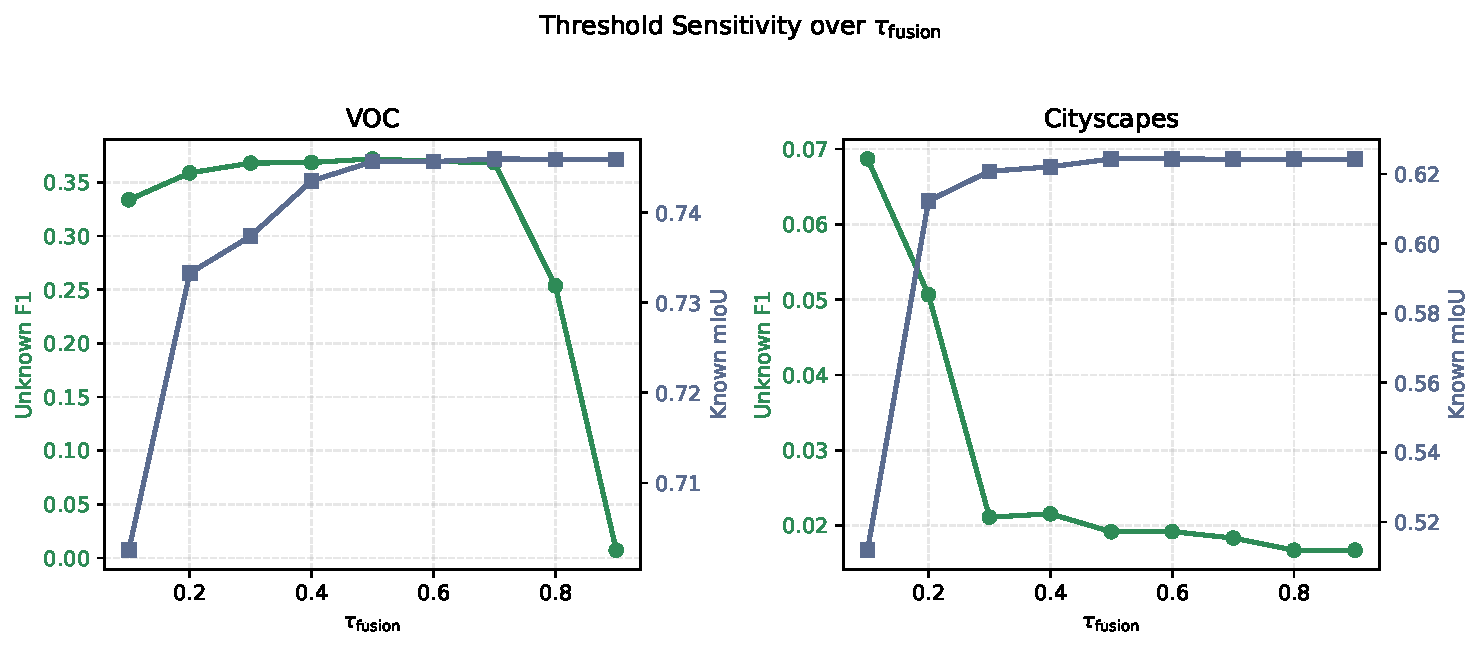
\includegraphics[width=\linewidth]{fig/fusion_sweep.pdf}
  \caption{Sensitivity of L2 to the fusion threshold $\tau_{\text{fusion}}$. VOC is broadly stable across a wide threshold range, whereas Cityscapes exhibits a sharper operating-point trade-off between Unknown F1 and Known mIoU.}
  \label{fig:supp-fusion-sweep}
\end{figure}

\subsection{Prompt-Form Ablation}
\label{sec:supp:prompt}

\begin{figure}[t]
  \centering
  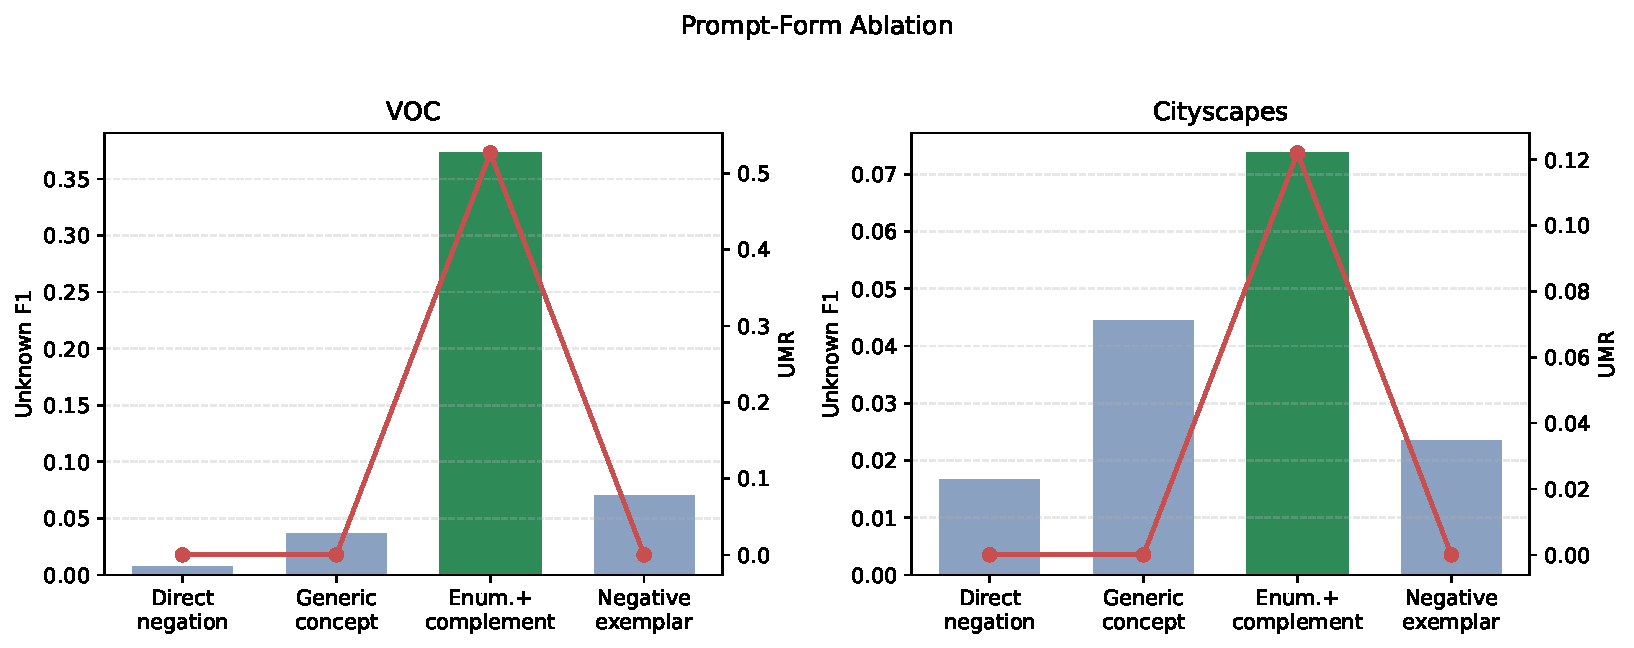
\includegraphics[width=\linewidth]{fig/prompt_form_ablation.pdf}
  \caption{Prompt-form ablation on VOC and Cityscapes. Bars show full-system Unknown F1 and the overlaid line shows prompt-level unknown-mask recall. Enumeration-then-complement is the only prompt form that produces a consistently usable structural signal.}
  \label{fig:supp-prompt-ablation}
\end{figure}

\section{SMIYC Trade-Off Visualization}
\label{sec:supp:smiyc}

\begin{figure*}[t]
  \centering
  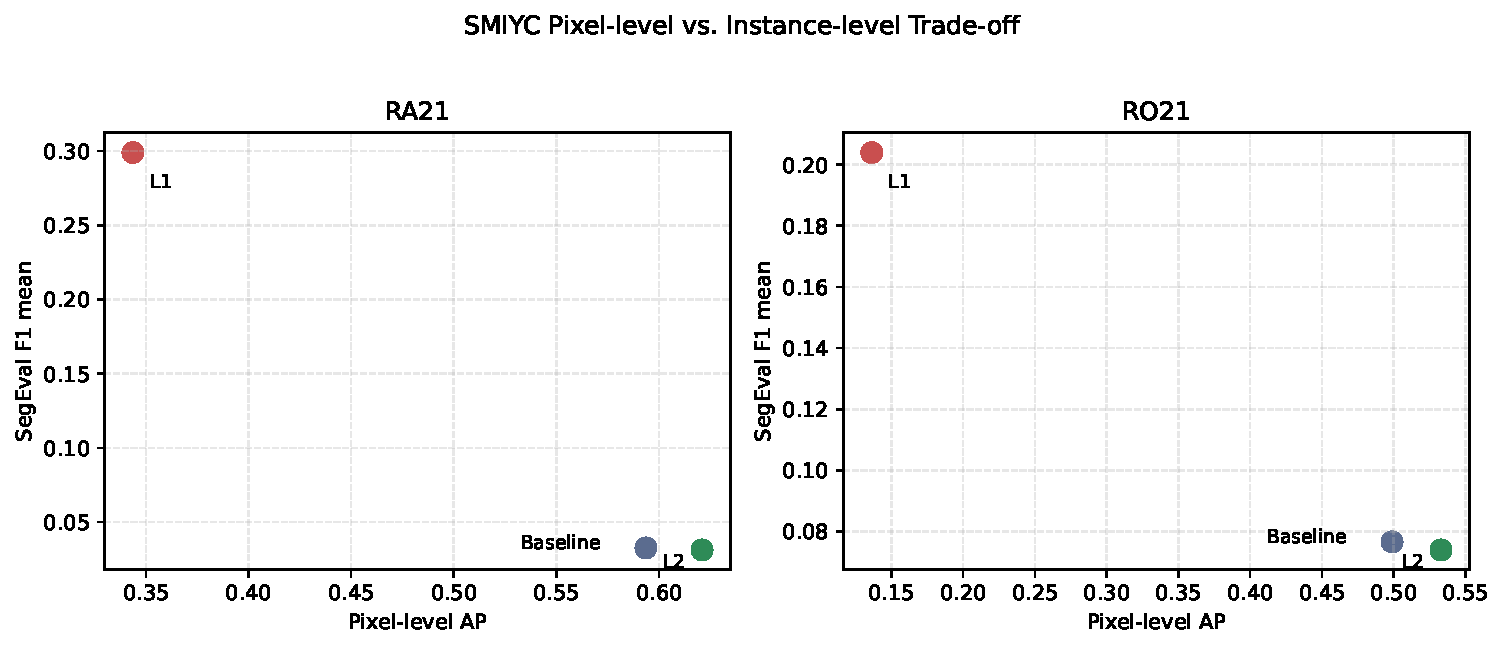
\includegraphics[width=\textwidth]{fig/smiyc_tradeoff.pdf}
  \caption{SMIYC pixel-level versus instance-level trade-off. Each point corresponds to Baseline, L1, or L2 on RoadAnomaly21 and RoadObstacle21. L2 moves toward better pixel-level AP, whereas L1 remains stronger on instance-level SegEval F1 mean, exposing the limitation of mean-score mask filtering.}
  \label{fig:supp-smiyc-tradeoff}
\end{figure*}

\end{document}
